\begin{sol}[1](Résolu par Matthias Schuller)

On a $3^{2n}=9^n$,
or $9 \equiv 2 [7]$,
donc pour tout $n \in \mathbb{N}$, $9^n \equiv 2^n [7]$,
donc $3^{2n}-2^n \equiv 0 [7]$.

\end{sol}

\begin{sol}[29](Résolu par Sébastien Labbé)

Soit $s=min(x,\frac{1}{x}+y, \frac{1}{y})$.
Pour $x=\sqrt{2}$ et $\frac{1}{y}=\sqrt{2}$, on a $\frac{1}{x}+y=\sqrt{2}$, donc $s=\sqrt{2}$.\\
De plus, si $x\leq \sqrt{2}$ ou $\frac{1}{y} \leq \sqrt{2}$, on a $s \leq \sqrt{2}$.\\
Sinon, on a $x> \sqrt{2}$ et $\frac{1}{y}>\sqrt{2}$, on a $\frac{1}{x}+y<\sqrt{2}$, donc $s<\sqrt{2}$.\\
Ainsi la valeur maximale de $s$ vaut $\sqrt{2}$.


\end{sol}

\begin{sol}[24](Résolu par Jules Bouton)

Soit $m,n \in \mathbb{N}$.n Notons $d= PGCD(m,n)$.
Deux cas sont \`a distinguer :
\begin{itemize}
	\item[$d \not =1$]
		Soit $r \in \mathbb{N}$ tel que $d$ ne divise pas $r$. Alors il n'existe pas $(a,b) \in \mathbb{Z}^2$ tel que $am+bn=r$, car sinon on aurait $d$ divise $a$ et $b$,
		donc $d$ divise $r$.
		Ainsi il ne peut pas exister de tel $N$.

	\item[$d=1$]
		D'apr\`es le th\'eror\`eme de Bezout, il existe $(a_0,b_0) \in \mathbb{Z}^2$ tel que $a_0m+b_0n=1$.
		Soit $r\in \mathbb{N}$. On a alors $a_0mr+b_0nr=r$
		Notons $a_1=a_0m$ et $b_1=b_0n$.
		Pour tout $k \in \mathbb{Z}$ on a $(a_1+kn, b_1-km)$ qui convient \'egalement. 
		Il suffit ainsi d'avoir pour un certain $k \in \mathbb{Z}$, $a_1+k_n \geq 0$ et $b_1-km \geq 0$, c'est-\`a-dire
		$k\geq -\frac{a}{n}$ et $k \leq \frac{b}{n}$.
		Il suffit donc pour qu'un tel $k$ existe que $-\frac{a}{n}+1 \leq \frac{b}{m}$,
		ce qui correspond \'a $nm \leq bn+am$, soit $nm \leq r$.
		$N=nm$ convient donc.
		
	

\end{itemize}



\end{sol}



\begin{sol}[34](Résolu par Rodion Zaystev)
On divise la figure

\[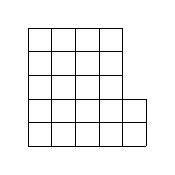
\begin{tikzpicture}[scale=0.3]
\draw (0, 0)--(0,5 );
\draw (1, 0)--(1,5 );
\draw (2, 0)--(2,5 );
\draw (3, 0)--(3,5 );
\draw (4, 0)--(4,5 );
\draw (5, 0)--(5,2 );

\draw(0,0)--(5,0);
\draw(0,1)--(5,1);
\draw(0,2)--(5,2);
\draw(0,3)--(4,3);
\draw(0,4)--(4,4);
\draw(0,5)--(4,5);
\end{tikzpicture}\]

en morceaux de forme 
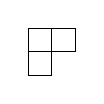
\begin{tikzpicture}[scale=0.3]
\draw(0,0)--(0,2);
\draw(1,0)--(1,2);
\draw(2,1)--(2,2);
\draw(0,0)--(1,0);
\draw(0,1)--(2,1);
\draw(0,2)--(2,2);
\end{tikzpicture}
et
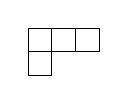
\begin{tikzpicture}[scale=0.3]
\draw(0,0)--(0,2);
\draw(1,0)--(1,2);
\draw(2,1)--(2,2);
\draw(3,1)--(3,2);
\draw(0,0)--(1,0);
\draw(0,1)--(3,1);
\draw(0,2)--(3,2);
\end{tikzpicture}.


Celle-ci est constituée de $22$ cases 
On note $x$ le nombre de morceaux de $3$ cases, et $y$ celui de ceux de $4$ cases.
On a alors $3x+4y=22$, et $x \geq 0$ et $y \geq 0$, donc $y \leq 5$.
Or $y$ est un entier, donc il n'y a que $6$ valeurs possibles de $y$:
\begin{itemize}
	\item[y=0:] Impossible car $3x=22$ avec $x$ entier
	\item[y=1:] $3x=18$ donc $x=6$
	\item[y=2:] Impossible car $3x=14$ avec $x$ entier
	\item[y=3:] Impossible car $3x=10$ avec $x$ entier
	\item[y=4:] $3x=6$ donc $x=2$
	\item[y=5:] Impossible car $3x=2$ avec $x$ entier
\end{itemize}
Ainsi les seules valeures possibles de $x$ sont $2$ et $6$.
Réciproquement, les deux figures suivantes montrent que ces $2$ valeurs conviennent effectivement.

\[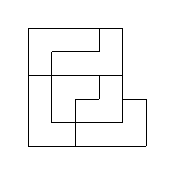
\begin{tikzpicture}[scale=0.3]
\draw (0, 0)--(0,5 );
\draw (1, 1)--(1,4 );
\draw (2, 0)--(2,2 );
\draw (3, 2)--(3,3 );
\draw (3, 4)--(3,5 );
\draw (4, 1)--(4,5 );
\draw (5, 0)--(5,2 );

\draw(0,0)--(5,0);
\draw(1,1)--(4,1);
\draw(2,2)--(3,2);
\draw(4,2)--(5,2);
\draw(0,3)--(4,3);
\draw(1,4)--(3,4);
\draw(0,5)--(4,5);
\end{tikzpicture}\]

\[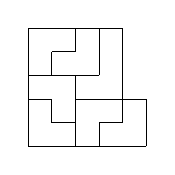
\begin{tikzpicture}[scale=0.3]
\draw (0, 0)--(0,5 );
\draw (1, 1)--(1,2 );
\draw (1, 3)--(1,4 );
\draw (2, 0)--(2,3 );
\draw (2, 4)--(2,5 );
\draw (3, 0)--(3,1 );
\draw (3, 3)--(3,5 );
\draw (4, 1)--(4,5 );
\draw (5, 0)--(5,2 );

\draw(0,0)--(5,0);
\draw(1,1)--(2,1);
\draw(3,1)--(4,1);
\draw(0,2)--(1,2);
\draw(2,2)--(5,2);
\draw(0,3)--(3,3);
\draw(1,4)--(2,4);
\draw(0,5)--(4,5);
\end{tikzpicture}\]

\end{sol}

\begin{sol}[62](Résolu par Vincent Geffroy)
On cherche \`a relier $n$ puits \`a $n$ villages sans que deux segments ne se croisent.
On remarque tout d'abord que lorsque deux chemins sont crois\'es et qu'on les d\'ecroise, par in\'egalit\'e triangulaire, la longueur des segments d\'ecroit strictement.
\[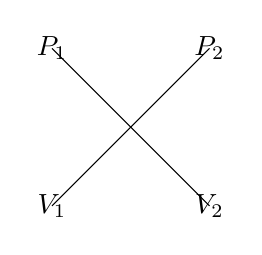
\begin{tikzpicture}[scale=1]
\draw (0, 0)--(2,2 );
\draw (2, 0)--(0,2 );
\node at (0,0) {$V_1$};
\node at (2,0) {$V_2$};
\node at (0,2) {$P_1$};
\node at (2,2) {$P_2$};

\end{tikzpicture}\]

\[\begin{tikzpicture}[scale=1]
\draw (0, 0)--(0,2 );
\draw (2, 0)--(2,2 );
\node at (0,0) {$V_1$};
\node at (2,0) {$V_2$};
\node at (0,2) {$P_1$};
\node at (2,2) {$P_2$};

\end{tikzpicture}\]

On sait qu'il n'existe qu'un nombre fini de mani\`eres de relier les $n$ puits aux $n$ villages (avec ou sans croisements), \`a chacune de ces mani\`eres, on associe la longueur totale des segments de la configuration. Il existe donc une configuration qui minimise cette longueur totale.
Montrons que dans celle-ci, aucun segment ne se croise.
En effet, si deux chemins se croisent, alors en les d\'ecroisant, on obtient une configuration de longueur plus petite, ce qui contredit la minimalit\'e de la configuration pr\'ec\'edente.
Ainsi le prince peut r\'eussir.




\end{sol}



\begin{sol}[69](Résolu par Pierre-Marie Esmenjaud et Thibaut Maron)

Soit $a,b,c$ les longueurs des côtés d'un triangle. Montrons que l'on a toujours $a^2b(a-b)+b^2c(b-c)+c^2a(c-a) \geq 0$.\\
On utilise la substitution de Ravi, il existe $x,y,z$ positifs tels que 
$a=x+y$,$b=y+z$, $c=z+x$.
En développant l'inégalité et en la simplifiant, on obtient alors
$2(x^3y+y^3x+z^3y-x^2yz-y^2xz-z^2xy) \geq 0$,
c'est-\`a-dire $x^3y+y^3x+z^3y \geq x^2yz+y^2xz+z^2xy$
Or les suites $(x^2,y^2,z^2)$ et $(yz,xz,xy)$ sont dans l'ordre opposé, donc par l'in\'egalit\'e de r\'eordonnement,
on a $x^2xy+y^2yz+z^2zy \geq x^2yz+y^2xz+z^2xy$, ce qui correspond \`a l'in\'egalit\'e initiale.

\end{sol}

\begin{sol}[99](Résolu par Baptiste Serraille)
		\definecolor{uuuuuu}{rgb}{0.26666666666666666,0.26666666666666666,0.26666666666666666}
		\definecolor{qqqqff}{rgb}{0.,0.,1.}
		\begin{tikzpicture}[line cap=round,line join=round,>=triangle 45,x=0.5cm,y=0.5cm]
		\clip(-4.8866410764292,-5.572904036609516) rectangle (24.92335892357077,7.055095963390474);
		\draw (3.38,4.66)-- (4.6,-3.1);
		\draw (4.6,-3.1)-- (13.6,-3.2);
		\draw (3.38,4.66)-- (13.6,-3.2);
		\draw(6.6073797978803945,-0.7786041073342618) circle (1.171777726594992cm);
		\draw (3.8617737962416823,1.595602738659465)-- (7.415842784909827,1.556113083229819);
		\draw (1.0600044164045799,-3.0606667157378284)-- (5.638808290575755,1.575857910944642);
		\draw (1.0600044164045799,-3.0606667157378284)-- (6.581341825154507,-3.1220149091683833);
		\draw (1.0600044164045799,-3.0606667157378284)-- (8.036095081092272,1.0790893016257088);
		\begin{scriptsize}
		\draw [color=qqqqff] (3.38,4.66)-- ++(-2.5pt,-2.5pt) -- ++(5.0pt,5.0pt) ++(-5.0pt,0) -- ++(5.0pt,-5.0pt);
		\draw[color=qqqqff] (3.5393589235707914,5.053095963390476) node {$A$};
		\draw [color=qqqqff] (4.6,-3.1)-- ++(-2.5pt,-2.5pt) -- ++(5.0pt,5.0pt) ++(-5.0pt,0) -- ++(5.0pt,-5.0pt);
		\draw[color=qqqqff] (4.199358923570791,-2.712904036609518) node {$B$};
		\draw [color=qqqqff] (13.6,-3.2)-- ++(-2.5pt,-2.5pt) -- ++(5.0pt,5.0pt) ++(-5.0pt,0) -- ++(5.0pt,-5.0pt);
		\draw[color=qqqqff] (13.747358923570783,-2.800904036609518) node {$C$};
		\draw [color=uuuuuu] (8.036095081092272,1.0790893016257088)-- ++(-2.5pt,-2.5pt) -- ++(5.0pt,5.0pt) ++(-5.0pt,0) -- ++(5.0pt,-5.0pt);
		\draw[color=uuuuuu] (8.445358923570787,1.3350959633904789) node {$E$};
		\draw [color=uuuuuu] (4.292261123652807,-1.1425789504473618)-- ++(-2.5pt,-2.5pt) -- ++(5.0pt,5.0pt) ++(-5.0pt,0) -- ++(5.0pt,-5.0pt);
		\draw[color=uuuuuu] (3.913358923570791,-0.9309040366095195) node {$F$};
		\draw [color=uuuuuu] (6.581341825154507,-3.1220149091683833)-- ++(-2.5pt,-2.5pt) -- ++(5.0pt,5.0pt) ++(-5.0pt,0) -- ++(5.0pt,-5.0pt);
		\draw[color=uuuuuu] (6.729358923570788,-2.734904036609518) node {$D$};
		\draw [color=uuuuuu] (1.0600044164045799,-3.0606667157378284)-- ++(-2.5pt,-2.5pt) -- ++(5.0pt,5.0pt) ++(-5.0pt,0) -- ++(5.0pt,-5.0pt);
		\draw[color=uuuuuu] (0.7233589235707943,-2.690904036609518) node {$T$};
		\draw [color=uuuuuu] (6.6334177706062825,1.5648066944998584)-- ++(-2.5pt,-2.5pt) -- ++(5.0pt,5.0pt) ++(-5.0pt,0) -- ++(5.0pt,-5.0pt);
		\draw [color=uuuuuu] (3.8617737962416823,1.595602738659465)-- ++(-2.5pt,-2.5pt) -- ++(5.0pt,5.0pt) ++(-5.0pt,0) -- ++(5.0pt,-5.0pt);
		\draw[color=uuuuuu] (4.023358923570791,1.9950959633904781) node {$H$};
		\draw [color=uuuuuu] (7.415842784909827,1.556113083229819)-- ++(-2.5pt,-2.5pt) -- ++(5.0pt,5.0pt) ++(-5.0pt,0) -- ++(5.0pt,-5.0pt);
		\draw[color=uuuuuu] (7.719358923570788,2.1930959633904776) node {$G$};
		\draw [color=uuuuuu] (5.638808290575755,1.575857910944642)-- ++(-2.5pt,-2.5pt) -- ++(5.0pt,5.0pt) ++(-5.0pt,0) -- ++(5.0pt,-5.0pt);
		\draw[color=uuuuuu] (5.783358923570789,1.9730959633904783) node {$M$};
		\draw [color=uuuuuu] (4.939888935469334,0.8681279248895978)-- ++(-2.5pt,-2.5pt) -- ++(5.0pt,5.0pt) ++(-5.0pt,0) -- ++(5.0pt,-5.0pt);
		\draw[color=uuuuuu] (4.595358923570791,1.3790959633904787) node {$T_1$};
		\end{scriptsize}
		\end{tikzpicture}
				
		La solution utilise deux résultats de géométrie projective avancés : 
		
		i) Pour un point et un cercle donnés, les deux points de contact avec les tangentes par ce point et deux points sur une sécantes sont en division harmonique
		
		ii) Le birapport de quatre points sur un cercle est égal au birapport des tangentes en ces points
		
		iii) Soient $A,B$ des points et $M$ le milieu de $[AB]$. Alors $A,B,M,\infty$ sont harmoniques. Réciproquement, si $A,B,M,\infty$ sont harmoniques, alors $M$ le milieu de $[AB]$.
		
		Début de la solution :
		
		Soit $T_1$ le point de contact de la tangente (autre que $(TC)$) au cercle inscrit. Et soit $M_1$ le point d'intersection de $TT_1$ avec $(GH)$. Montrons que $M_1$ est le mileu de $(GH)$.
				
		D'après i) $T_1 F E D$ sont en division harmonique
		
		D'après ii) $$-1 =b_{T_1,D,F,E}=b_{T_1M_1,DB,FH,EG}=b_{M_1,\infty,H,G}$$
		
		Donc, d'après iii), $M_1$ est bien le milieu de $[HG]$.
\end{sol}

\begin{sol}[130](Résolu par Thibaut Maron)

Soit $x_1,x_2,\dots,x_{13}$ $13$ r\'eels deux \`a deux distincts.\\
La fonction tangente réalise une surjection (en fait une bijection) de $]-\frac{\pi}{2},\frac{\pi}{2}[$ dans $\mathbb{R}$, donc il existe $13$ réels $a_1,a_2,\dots,a_{13}$ appartenant tous \`a $]-\frac{\pi}{2},\frac{\pi}{2}[$ (intervalle de largeur $\pi$),
vérifiant $\forall i \in [[1,13]], \tan(a_i)=x_i$. \\
Or, par le principe des tiroirs, il existe $i$ et $j$ distincts tels que $ 0 \leq a_i-a_j \leq \frac{\pi}{12}$
Or la fonction tangente est croissante sur $]-\frac{\pi}{2},\frac{\pi}{2}[$, donc on peut composer l'in\'egalit\'e pr\'ec\'edente par tangente, \\
on obtient ainsi $\tan(0) \leq \tan(a_i-a_j) \leq \tan(\frac{\pi}{12})$, \\
en appliquant une formule de trigonométrie, \\
on a donc $0 \leq \frac{\tan(a_i)-\tan(a_j)}{1+\tan(a_i)\tan(a_j)} \leq 2-\sqrt{3} $ \\
Or $\forall i \in [[1,13]], \tan(a_i)=x_i$, \\
ainsi $0 \leq \frac{x_i-x_j}{1+x_i x_j} \leq 2-\sqrt{3}$,
ce qui conclut.

\end{sol}

\begin{sol}[1](Résolu par ....)
Lorem Ipsum
\end{sol}
